\section{Results} \label{sec:results}

\subsection{Main Result} \label{sec:main}

The main result of this paper is that we can approximate $\hbn$ very efficiently, and that this approach outperforms a more \naive approach of a typical deconvolution filter, half-wave rectified (i.e., setting everything below zero equal to zero).  Fig. \ref{fig:woopsi_inf} depicts a simulation showing this result. Clearly, the \foopsi filter is outperforming the optimal linear deconvolution filter (also called a Wiener filter).  The Wiener filter implicitly approximates the Poisson spike rate with a Gaussian spike rate (see Appendix for details). While a Gaussian well approximates a Poisson distribution when rates are about $10$ spikes per frame, this example is obviously very far from that regime, and so the Gaussian approximation does very poorly. Furthermore, the Gaussian approximation allows for the inferred spike train to include negative numbers, which we do not want, as spike trains are non-negative entities.  To counteract the negative values, the Wiener filter then infers large positive values, contributing to a ``ringing'' effect.  The non-negative constraint imposed by the \foopsi filter ensures that such ringing does not take place.  Finally, by utilizing Gaussian elimination and interior-point methods, as described in the Methods section, the computational complexity of \foopsi filter is the same as an efficient implementation of the Wiener filter.  


\begin{figure}[h!]
\centering 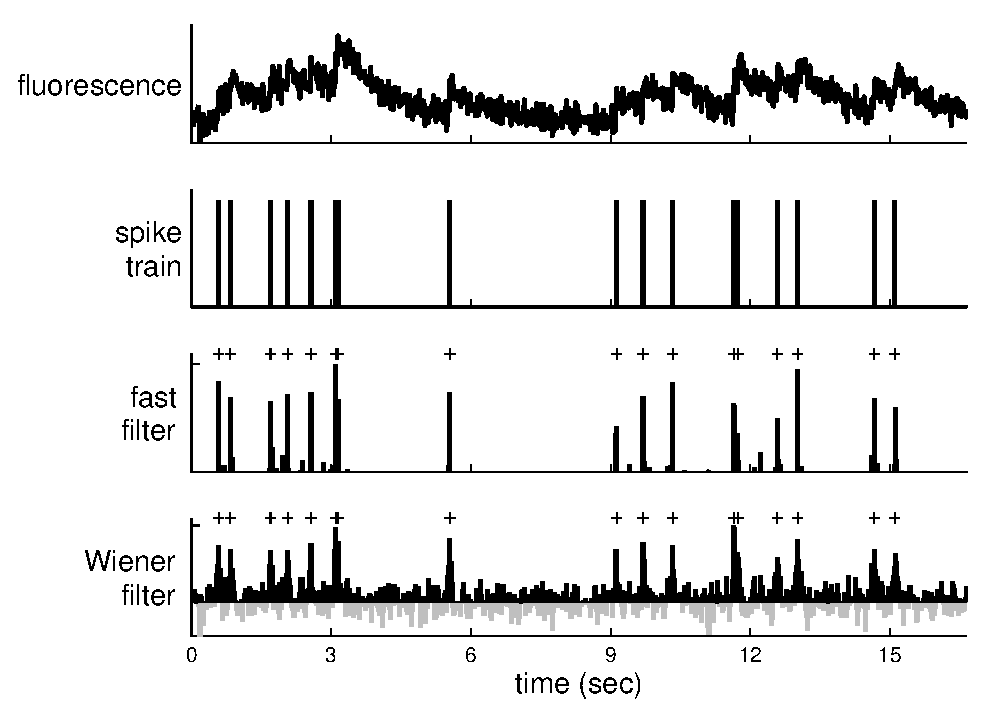
\includegraphics[width=.9\linewidth]{../figs/woopsi_inf}
\caption{The \foopsi filter significantly outperforms the optimal linear deconvolution (aka, Wiener) filter on typical simulated data-sets. Top panel: fluorescence trace.  Second panel: spike train.  Third panel: \foopsi filter inference.  Bottom panel: Wiener filter inference.  Gray '$+$'s in bottom two panels indicate true spike times.  Simulation details: $T=2930$ time steps, $\Del=5$ msec, $\alpha=1$, $\beta=0$, $\sig=0.3$, $\tau=1$ sec, $\lam=1$ Hz.} \label{fig:woopsi_inf}
\end{figure}


In the above, we assumed that we knew the model parameters of interest.  However, in the general case, the parameters are unknown, and must therefore be estimated from the data.  In Section \ref{sec:learn} we described how the parameters of our model may be estimated directly from the observations.  Importantly, this obviates the need to conduct joint imaging and electrophyiological experiments to obtain ``training'' data, as the developed approach is fully unsupervised.  Figure \ref{fig:woopsi_learn} shows another simulated example; in this example, however, the parameters are estimated from the observed fluorescence trace.  Again, it is clear that the \foopsi filter far outperforms the Wiener filter.

\begin{figure}[h!]
\centering 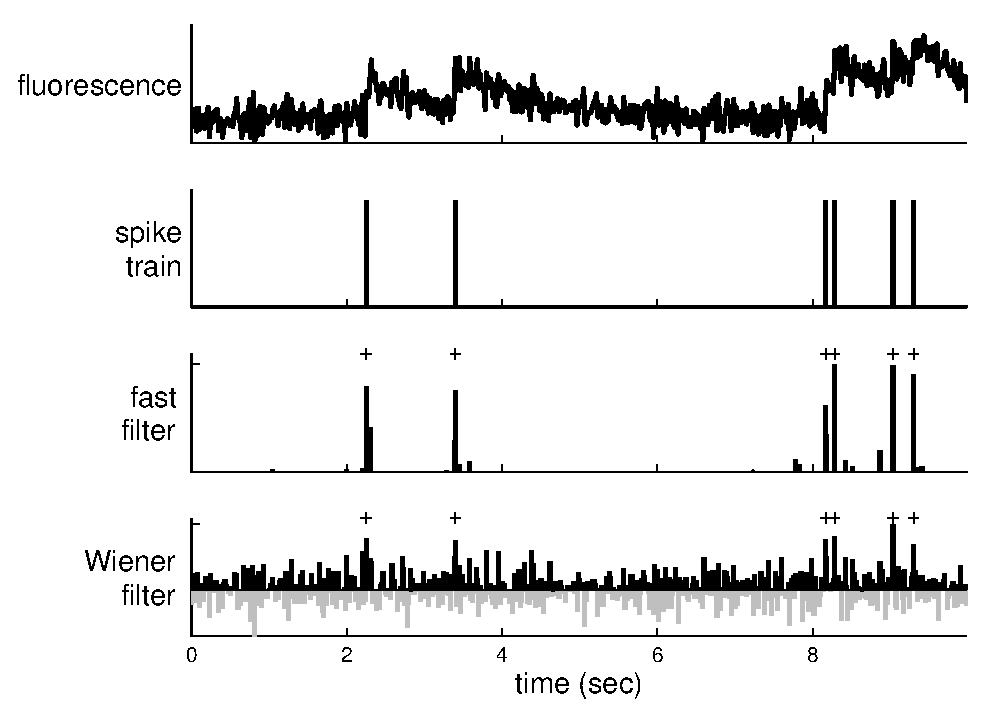
\includegraphics[width=.9\linewidth]{../figs/woopsi_learn}
\caption{The \foopsi filter significantly outperforms the Wiener filter, even when estimating the parameters only from the observed data.  Simulated details as in Figure \ref{fig:woopsi_inf}.} \label{fig:woopsi_learn}
\end{figure}

Given the above two results, we then applied this \foopsi filter to real data.  More specifically, by simultaneously recording electrophysiologically and imaging, we can determine the true spike times, and then compare the accuracy of the two filters.  Figure \ref{fig:woopsi_data} shows similar result for this typical in vitro data-set.  These results are typical of the 12 joint electrophysiological and imaging experiments conducted (not shown). Note that the first few ``events'' are actually pairs of spikes, which is reflected in the inferred spike trains.

\begin{figure}[h!]
\centering 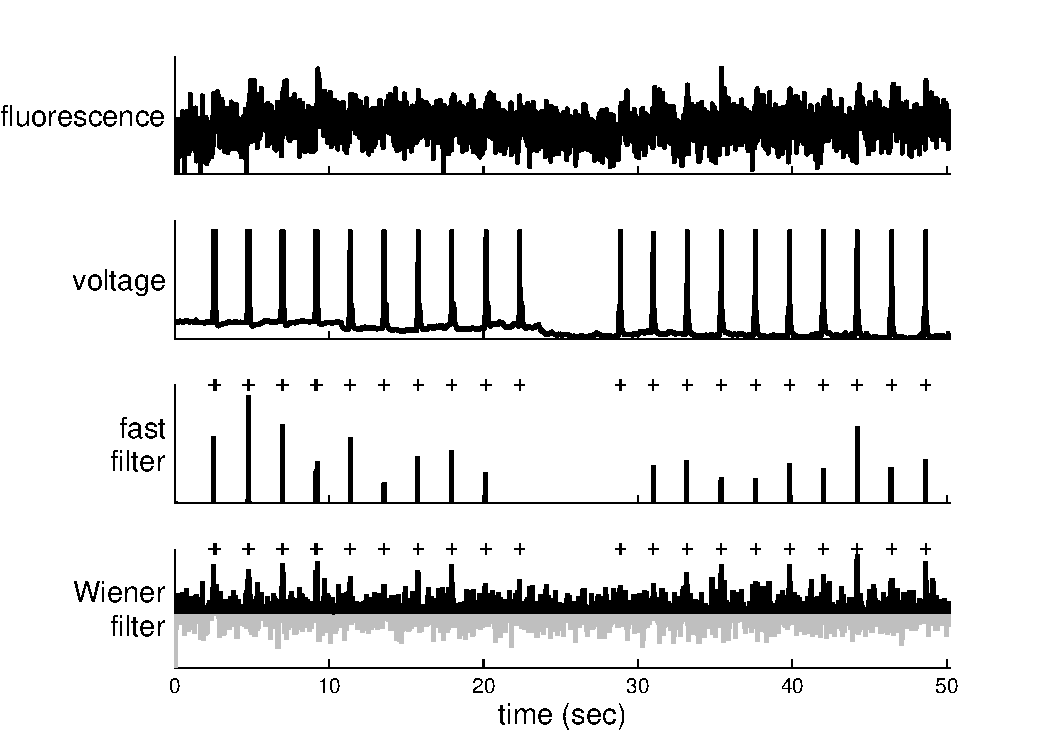
\includegraphics[width=.9\linewidth]{../figs/woopsi_data4}
\caption{The \foopsi filter significantly outperforms the Wiener filter on typical in vitro data-sets.  Note that all the parameters for both filters were estimated from the data.} \label{fig:woopsi_data}
\end{figure}

\subsection{Online analysis of spike trains using the \foopsi filter}

A central aim for this work was the development of a algorithm that infers spikes sufficiently efficiently to use online while imaging a large population (eg, $\approx 100$) of neurons.  Figure \ref{fig:pop} shows the result of running \foopsi on 136 neurons, recorded simultaneously, as described in the Methods section.  Note that the filtered fluorescence signals much more clearly show fluctuations in spiking. These spike trains were inferred in approximately real time, meaning that one could infer spike trains for the past experiment while conducting the subsequent experiment.


\begin{figure}[h!]
\centering 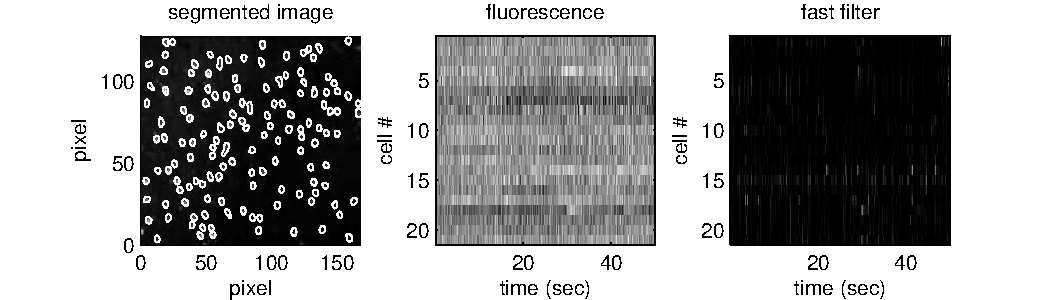
\includegraphics[width=.9\linewidth]{../figs/pop}
\caption{Applying the \foopsi filter in real time to a large population of neurons imaged simultaneously.  The inferred spike trains convey much more clearly the neural activity.  Left panel: Mean segmented image field.  Middle panel: example fluorescence traces.  Right panel: \foopsi filter output corresponding to each associated trace.} \label{fig:pop}
\end{figure}


\subsection{Improving inference results}

In Section \ref{sec:model}, we described a simple principled first-order model relating the spike trains to the fluorescence trace.  A number of the simplifying assumptions that we made above can be straightforwardly relaxed.  We tried relaxing three in particular: the linearity between calcium and fluorescence, the Gaussianity of the noise on the fluorescence measurements, and the static nature of the prior, $\lam$.  Combining all three of these modifications yields a more powerful model:


\begin{align}
	F_t &\sim \text{Poisson}(\alpha S(C_t) + \beta) \label{eq:nonlin} \\
	% C_t &= (1-\Del/\tau)C_{t-1} + n_t
	n_t &\sim \text{Poisson}(\lam_t \Del),
\end{align}

\noindent where the dynamics for calcium are as before, and we take $S(C_t)=\frac{C_t}{C_t + k_d}$ to be the standard Hill equation \cite{PologrutoSvoboda04}.  To modify our \foopsi filter to be optimal for this new model, we must simply compute the gradient and Hessian for the MAP estimate of this new model.  Note that both the Poisson observation assumption and the time-varying assumption maintain the log-concavity of the posterior, meaning that by using Newton-Raphson, we are still guaranteed to converge to the globally optimal solution.   

Unfortunately, using this more powerful model did not result in substantial inference improvements for simulated or in vitro data (not shown).  This is possibly due to approximating the Poisson distribution governing spiking with an exponential distribution.  This approximation is required to ensure concavity of the posterior.  In previous work, we developed a sequential Monte Carlo (SMC) method to infer spike trains \cite{VogelsteinPaninski09}, that does not require such an assumption. Like the fast filter, the SMC filter estimates the model parameters in a completely unsupervised fashion, ie, from the fluorescence observations, using an expectation-maximization algorithm.  Previously, we initialized parameters for the SMC filter based on other data-sets.  While effective, this initialization was often far from the final estimates, and therefore, required a relatively large number of iterations (eg, 20-25) before converging.  Thus, we reasoned that we could use the \foopsi filter to improve the initial parameter estimates, and reduce the required number of iterations.  Indeed, Figure \ref{fig:smc_init} shows how the SMC filter outperforms the \foopsi filter on in vitro data, and only required $3$--$5$ iterations to converge.  Note that the first few events are individual spikes, resulting in relatively small fluorescence fluctuations, whereas the next events are actually spike doublets, causing a much larger fluorescence fluctuation.  Only the SMC filter picks up the individual spikes in this trace, a result typical when the effective signal-to-noise ratio (SNR) is so poor.  Thus, these two inference algorithms are complementary: the \foopsi filter can be used for rapid, online inference, and for initializing the SMC filter, which can then be used to further refine the spike train estimate.

\begin{figure}[h!]
\centering 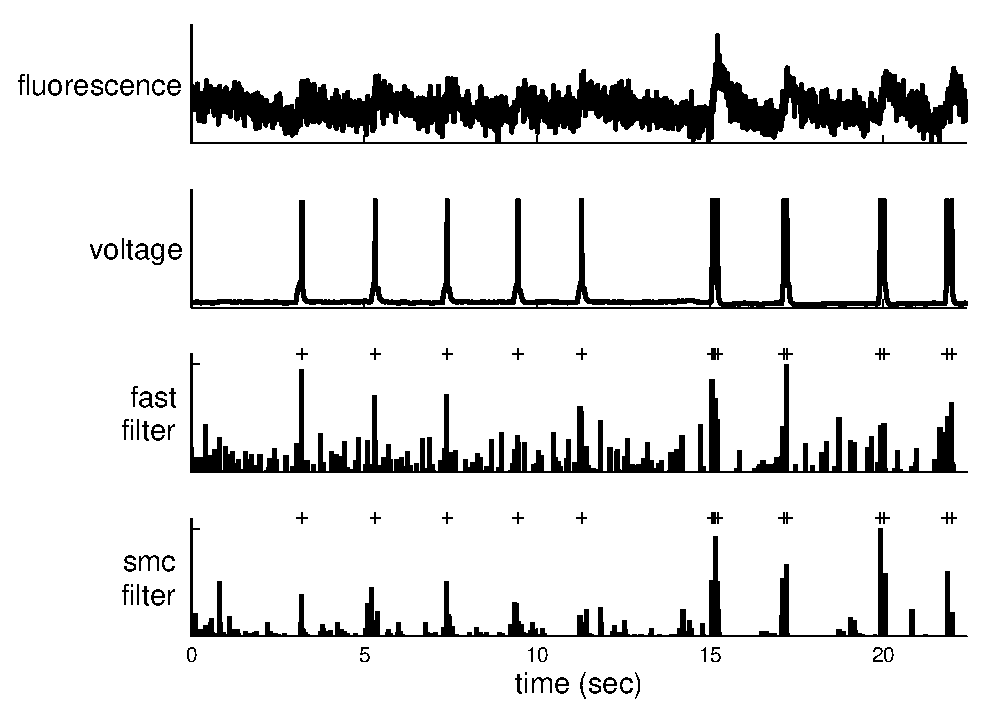
\includegraphics[width=.9\linewidth]{../figs/smc_init12}
\caption{The \foopsi filter effectively initializes the parameters for the SMC filter (which outperforms the \foopsi filter), significantly reducing the number of expectation-maximization iterations to convergence.  Note that the ordinate on the bottom panel corresponds to the probability of a spike having occurred in each frame.} \label{fig:smc_init}
\end{figure}

\subsection{Spatial filter}

In the above, we assumed that the data was a one-dimensional fluorescence trace.  In actuality, the data is a time series of images, which are first segmented into regions-of-interest (ROI), and typically, then averaged, to obtain $F_t$.  In theory, one could improve the effective SNR of the fluorescence trace by scaling each pixel relative to one another.  In particular, pixels not containing any information about calcium fluctuations can be ignored, and pixels that are approximately anti-correlated with one another could have weights with opposing signs.  

Figure \ref{fig:spatial} demonstrates the potential utility of this approach.  The top row shows different depictions of an ROI containing a single neuron.  On the far left panel is the true spatial filter for this neuron.  This particular spatial filter was chosen based on our experience analyzing both in vitro and in vivo movies; often, it seems that the pixels immediately around the soma are anti-correlated with those in the soma.  This effect is possibly due to the influx of calcium from extracellular space immediately around the soma.  This simulated movie is relatively noisy, as indicated by the second panel, which depicts an exemplary image frame.  The standard approach, given such a noisy movie, would be to first segment the movie to find an ROI corresponding to the soma of this cell, and then spatially average all the pixels found to be within this ROI.  The third panel shows this ``typical spatial filter''.  The forth panel shows the mean frame, ie, $\langle \vbF \rangle_t$.  Clearly, this mean frame is very similar to the true spatial filter.

The bottom panels of Figure \ref{fig:spatial} depict the effect of using the true spatial filter, versus the typical one. The left side shows the fluorescence trace and its associated spike inference obtained from using the typical spatial filter.  The right side shows the same when using the true spatial filter.  Clearly, the true spatial filter results in a much cleaner fluorescence trace and spike inference.  


\begin{figure}[h!]
\centering 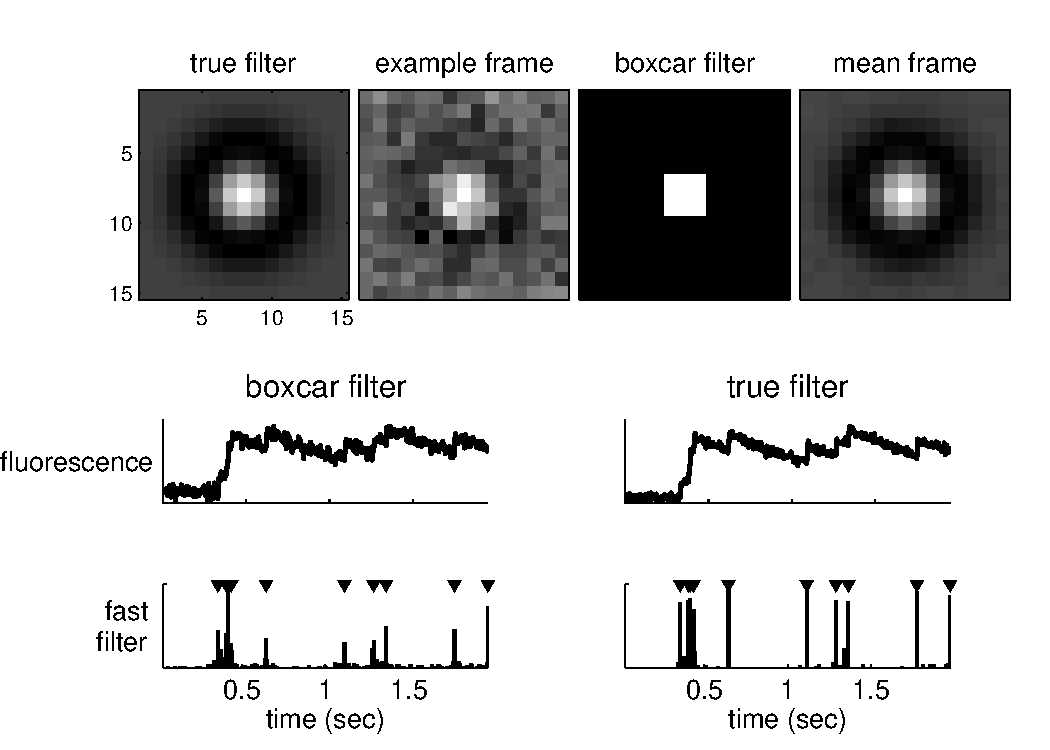
\includegraphics[width=.9\linewidth]{../figs/spatial2}
\caption{A simulation demonstrating that using a better spatial filter can significantly enhance the effective SNR (see Supplementary Movie 1 for the full movie associated with this simulation). We modeled the true spatial filter as a sum of Gaussians: a positively weighted small variance Gaussian, and a negatively weighted large variance Gaussian (both with the same mean).  Top row far left: true spatial filter.  Top row second from left: example frame (frame number 100). Top row second from right: typical spatial filter.   Top row far right: mean frame.  Middle row left: fluorescence trace using typical spatial filter. Bottom row left: \foopsi filter output using typical spatial filter.  Middle row right: fluorescence trace using true spatial filter.  Bottom right: \foopsi filter output using true spatial filter. Simulation details: $\valpha=\mN(\ve{0},2 \bI)-1.1 \mN(\ve{0},2.5 \bI)$ where $\mN(\ve{mu},\ve{\Sig})$ indicates a Gaussian with mean $\ve{\mu}$ and covariance matrix $\ve{\Sig}$, $\bbeta=1$, $\tau=0.85$ sec, $\lam=5$ Hz.} \label{fig:spatial} 
\end{figure}



\subsection{Overlapping spatial filters}


The above shows that if a ROI contains only a single neuron, we can enhance the effective SNR by spatially filtering.  However, this analysis assumes that only a single neuron is in the ROI.  Often, neural spatial filters are overlapping, or nearly overlapping, making the segmentation problem even more difficult.  Therefore, it is desirable to have an ability to crudely segment, yielding only a few neurons in each ROI, and then spatially filtering within each ROI to pick out the spike trains from each neuron.  We can do this in a principled manner by generalizing our model as described in Section \ref{sec:methods:overlapping}.  Figure \ref{fig:spatial_multi_inf} shows an example of this approach on simulated data. Note that the spatial filters are sufficiently overlapping that some ``bleed-though'' can be seen across the traces.  


\begin{figure}[h!]
\centering 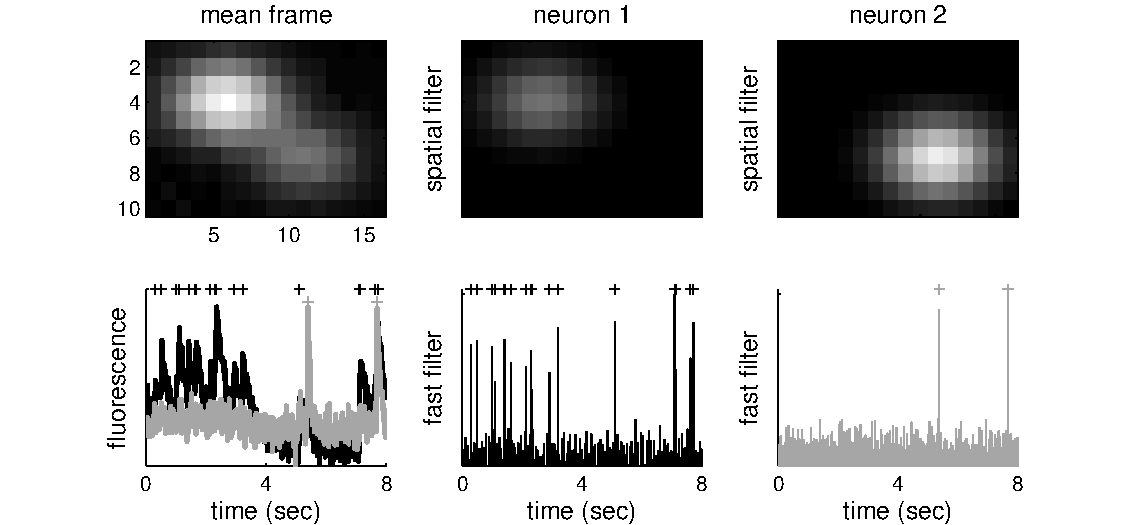
\includegraphics[width=.9\linewidth]{../figs/spatial_multi_inf}
\caption{Simulation showing that even when two neurons' spatial filters are overlapping, one can separate the two signals by spatial filtering. Simulation details: $\valpha^1=\mN([-1.8 1.8],2 \bI)\, \valpha^2=\mN([1.8 -1.8],5 \bI)$, $\bbeta=[1 1]\T$, $\tau=[0.5 0.5]\T$ sec, $\lam=[1.5 1.5]$ Hz.} \label{fig:spatial_multi_inf}
\end{figure}

While Figure \ref{fig:spatial_multi_inf} shows that one could separate the signals if the spatial filters of the neurons were known, FIgure \ref{fig:spatial_multi_learn} shows that we can estimate the spatial filters, using only the fluorescence movie, using the approach described in Section \ref{sec:methods:overlapping}.


\begin{figure}[h!]
\centering 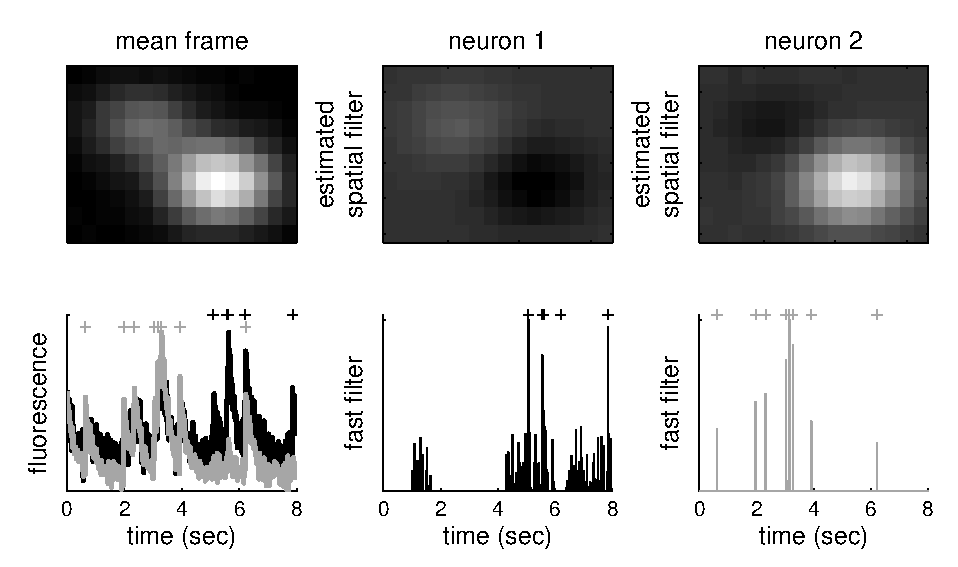
\includegraphics[width=.9\linewidth]{../figs/spatial_multi_learn}
\caption{Simulation showing that even when two neuron's spatial filters are largely overlapping, we can infer the spatial filter of each, to separate the two signals. Simulation details as above.} \label{fig:spatial_multi_learn}
\end{figure}

